\begin{XeClass}{FsShellPermissions}
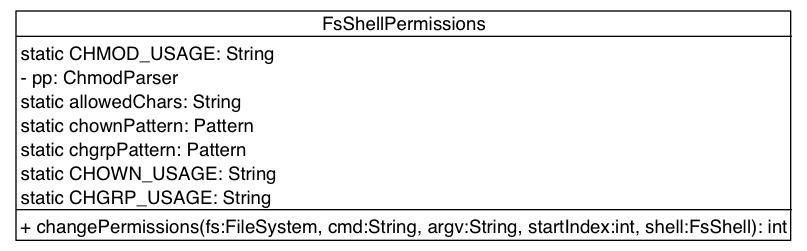
\includegraphics[width=10cm]{cdig/FsShellPermissions.png}
     
 FsShellPermissions类是将文件操作与命令行关联起来的类
 因为FsShell类越来越大,所以将FsShellPermissions类单独分离出来
 FsShellPermissions类中有三个静态内部类,分别是ChmodHandler,ChownHandler和ChgrpHandler
 还有一个静态方法changePermissions,将三个静态内部类的情况与命令行关联起来使用

    \begin{XeMethod}{}{int}{changePermissions}
         
 静态方法changePermissions,将三个静态内部类的情况与命令行关联起来使用
 当cmd匹配上-chmod,调用ChmodHandler(fs, argv[startIndex++])构造函数并将对象赋值给handler
 当cmd匹配上-chown,调用ChownHandler(fs, argv[startIndex++])构造函数并将对象赋值给handler
 当cmd匹配上-chgrp,调用ChgrpHandler(fs, argv[startIndex++])构造函数并将对象赋值给handler

    \end{XeMethod}

    \begin{XeInnerClass}{ChmodHandler}
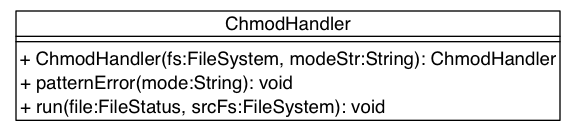
\includegraphics[width=10cm]{cdig/ChmodHandler.png}
        
        \begin{XeMethod}{}{ChmodHandler}{ChmodHandler}
             
 ChmodHandler继承自CmdHandler,ChmodHandler构造函数调用父类的构造函数并传入"chmod"和fs
 同时传入modeStr生成ChmodParser对象赋值给FsShellPermissions类的静态变量ChmodParser pp

        \end{XeMethod}

        \begin{XeMethod}{\XePrivate}{void}{patternError}
             
 当模式发生错误匹配不上时候抛出带有特定信息异常

        \end{XeMethod}

        \begin{XeMethod}{\XePublic}{void}{run}
             
 Override父类run方法从ChmodParser对象pp获得权限(写入权限,读取权限,操作权限)

        \end{XeMethod}

    \end{XeInnerClass}
    \begin{XeInnerClass}{ChownHandler}
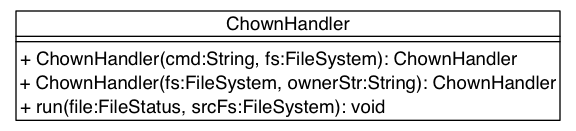
\includegraphics[width=10cm]{cdig/ChownHandler.png}
        
        \begin{XeMethod}{\XeProtected}{ChownHandler}{ChownHandler}
             
 ChownHandler继承自CmdHandler,protected继承ChownHandler构造函数调用父类的构造函数并传入cmd和fs

        \end{XeMethod}

        \begin{XeMethod}{}{ChownHandler}{ChownHandler}
             
 ChownHandler继承自CmdHandler,ChownHandler构造函数调用父类的构造函数并传入"chown"和fs
 chownPattern使用正则表达式匹配ownerStr并赋值给matcher,mathcer内部存有若干组匹配上的结果
 将第二组matcher.group(1)结果赋值给这个类的owner,将第四组结果matcher.group(3)赋值给这个类的group

        \end{XeMethod}

        \begin{XeMethod}{\XePublic}{void}{run}
             
 通过从file.getOwner()和file.getGroup()中取值分别与owner和group比较
 并将结果分别赋值给newOwner和newGroup
 当newOwner和newGroup其中一个为空,则从file.getOwner()和file.getGroup()取值
 在srcFs中调用setOwner(file.getPath(), newOwner, newGroup)方法

        \end{XeMethod}

    \end{XeInnerClass}
    \begin{XeInnerClass}{ChgrpHandler}
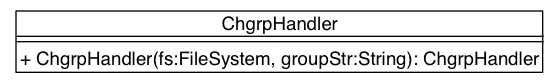
\includegraphics[width=10cm]{cdig/ChgrpHandler.png}
        
        \begin{XeMethod}{}{ChgrpHandler}{ChgrpHandler}
             
 ChgrpHandler继承自ChownHandler,ChgrpHandler构造函数调用父类的构造函数并传入chgrp和fs
 chgrpPattern使用正则表达式匹配groupStr并赋值给matcher,mathcer内部存有若干组匹配上的结果
 将第二组结果matcher.group(1)赋值给这个类的group

        \end{XeMethod}

    \end{XeInnerClass}
\end{XeClass}
